% !TEX root = paper.tex
\doclearpage
\section{Arithmetization}
\label{sec:arithmetization}


We now describe how we represent columns and tables as polynomials for use with the PIOPs of the following sections. 
We briefly review the general arithmetization of tables and columns in \cref{sec:general-approach}, which we adopt from $\truthtable$~\cite{cryptoeprint:2026/1260}, and then turn in \cref{sec:string-arith} to the arithmetization of strings---the focus of our paper and absent from $\truthtable$.

\subsection{General Approach}
\label{sec:general-approach}
Throughout, tables and columns are encoded as multilinear polynomials over the Boolean hypercube $\BoolHCube{\mu}$, with arithmetic in a finite field $\F$ of large prime characteristic $p$.

\parhead{Notation: arithmetized objects}
A concrete table or column is written plainly as $\Table$ or $\col$, and its \emph{arithmetized} polynomial form carries a hat, $\hat{\Table}$ or $\hat{\col}$. A concrete object is indexed by integers in square brackets, as in $\col[i]$ or $\Table.\key[i]$ for $i \in [|\Table|]$, whereas its arithmetization is evaluated at hypercube points in parentheses, as in $\hat{\Table}.\key(x)$ for $x \in \BoolHCube{\mu}$.

\parhead{Representing table data as field elements}
We map each column into the prime field $\F$ according to its declared type. For all non-string types---integers, booleans, durations, intervals, dates, and timestamps---we follow $\truthtable$~\cite{cryptoeprint:2026/1260}, to which we refer the reader for the encodings.
The encoding of strings as field elements is the subject of \cref{sec:string-arith}.

\parhead{Columns}
A column $\col$ of $n$ entries lives in $\BoolHCube{\mu}$ for any $\mu \ge \lceil \log_2 n \rceil$, and its arithmetization splits into two multilinear polynomials, $\hat{\col} := (\hat{\col}.\act,\, \hat{\col}.\data)$. The \emph{activator} $\hat{\col}.\act \colon \F^{\mu} \to \{0,1\}$ flags the $n$ \emph{active} indices---those carrying real rows rather than padding---while the \emph{data} polynomial $\hat{\col}.\data \colon \F^{\mu} \to \F$ holds the entries at those indices. Where the column is clear from context, we abbreviate the two to $\act$ and $\data$.

\parhead{Tables}
A $k$-column table $\Table$ with $n$ rows arithmetizes to $\hat{\Table} := (\hat{\Table}.\act,\, [\hat{\Table}.\data_1, \dots, \hat{\Table}.\data_k])$: a single activator $\hat{\Table}.\act$, active at $n$ points of $\BoolHCube{\mu}$, shared across all $k$ data polynomials. Each active point $x$---one with $\hat{\Table}.\act(x) = 1$---then yields a row $(\hat{\Table}.\data_1(x),\dots,\hat{\Table}.\data_k(x))$ of $\Table$. A column is just the $k=1$ case, and we reuse the $\hat{\Table}.\act$, $\hat{\Table}.\data_i$ notation for tables.

\parhead{Active indices and layouts.}
The \emph{active set} of $\hat{\col}$ (or $\hat{\Table}$) gathers its active points, $\actset(\hat{\col}) := \{x \in \BoolHCube{\mu} \mid \hat{\col}.\act(x) = 1\}$, and for a value $k \in \F$ we single out those carrying it as $\actset_k(\hat{\col}) := \{x \in \actset(\hat{\col}) \mid \hat{\col}.\data(x) = k\}$.

We use one of two layouts for the active set. In the default \emph{contiguous} layout, $\actset(\hat\Table) = \{0, \dots, n - 1\}$, so the activator is the closed-form $n$-contiguous polynomial $\contig_{\mu,n}$ (\cref{sec:prelims}) that the prover need neither commit to nor prove boolean. In the \emph{sparse} layout the active indices are scattered arbitrarily, and the prover must commit to the activator and prove its booleanity.


\parhead{Arithmetized relations}
Every operator PIOP proves membership in a \emph{table language}
$\Language{\op} = \{(x, \{\hat{\TableIn}\}, \{\hat{\TableOut}\})\}$, the input and output tables linked by the operator $\op$. Its \emph{arithmetized} counterpart replaces each concrete table with its polynomial form, $
\hat{\mathcal{L}}_\op := \{
    (\NPInstance = x,
    \NPInstancey = (\{\hat{\TableIn}\}, \hat{\TableOut}))
  \;|\;
  ((x, \{\TableIn\}, \TableOut), \bot ) \in \Language{\op}
\}
$,
where each $\hat{\Table} \in \{\hat{\TableIn}\} \cup \{\hat{\TableOut}\}$ is the arithmetization of the corresponding concrete table $\Table$.

\subsection{String Arithmetization}
\label{sec:string-arith}

We now describe how we arithmetize a string-typed column. This string arithmetization is a contribution of our work, and is designed so that the PIOP protocols of the following sections can operate directly on the contents of the strings.

We start with the approach of $\truthtable$~\cite{cryptoeprint:2026/1260} which arithmetizes a string-typed column as a single hash column $(\act,\mathsf{h})$, which acts as a black box handle to the strings and allows no white-box operation on the strings. We denote this as our main column. However, to enable white-box operations on the string contents, we introduce \emph{auxiliary columns}. The auxiliary columns are augmented to the hash column and come in two types with two different lengths:

\parhead{Type 1: String-level auxiliary columns} These are columns of length $N$---the length of the hash column, with one entry per string:
\begin{itemize}[nosep]
    \item \emph{Length column $\mathsf{l}$}, with $\mathsf{l}[i]$ being the length of the $i$-th string in $\col$.
    \end{itemize}
    \parhead{Type 2: Character-level auxiliary columns} These are columns of length $M := \sum_{s \in \col} |s|$, the total number of characters in the column:
   \begin{itemize}[nosep]
    \item \emph{Character column $\mathsf{char}$} contains the individual characters of all strings in $\col$ concatenated to each other.
    \item \emph{Origin index column $\mathsf{orig\text{-}ind}$}, with $\mathsf{orig\text{-}ind}[j]$ being the index of the string in $\col$ to which the $j$-th character of $\mathsf{char}$ belongs.
    \item \emph{Internal index column $\mathsf{int\text{-}ind}$}, with $\mathsf{int\text{-}ind}[j]$ being the position of the $j$-th character of $\mathsf{char}$ within its own string, counting from $0$. Equivalently, $\mathsf{int\text{-}ind}$ resets to $0$ at every string boundary and increments by one across the characters of each string.
    \item \emph{Character activator column $\mathsf{char\text{-}act}$}, with $\mathsf{char\text{-}act}[j]$ being $1$ if the $j$-th character of $\mathsf{char}$ is active, and $0$ otherwise.
    \item \emph{Boundary marker column $\mathsf{bnd}$}, with $\mathsf{bnd}[j]$ being $1$ if the $j$-th character of $\mathsf{char}$ is the first character of a string (a string boundary), and $0$ otherwise. \ali{This can be potentially removed from the arithmetization and be sent from the prover as int-ind==0 indicator. However, it comes with online prover cost.}
    \end{itemize}
\cref{fig:string-arith-example} illustrates this arithmetization on a sample four-row string-typed column.

\ifsp\begin{figure*}[tp]\else\begin{figure}[h!]\fi
\centering
\resizebox{\textwidth}{!}{%
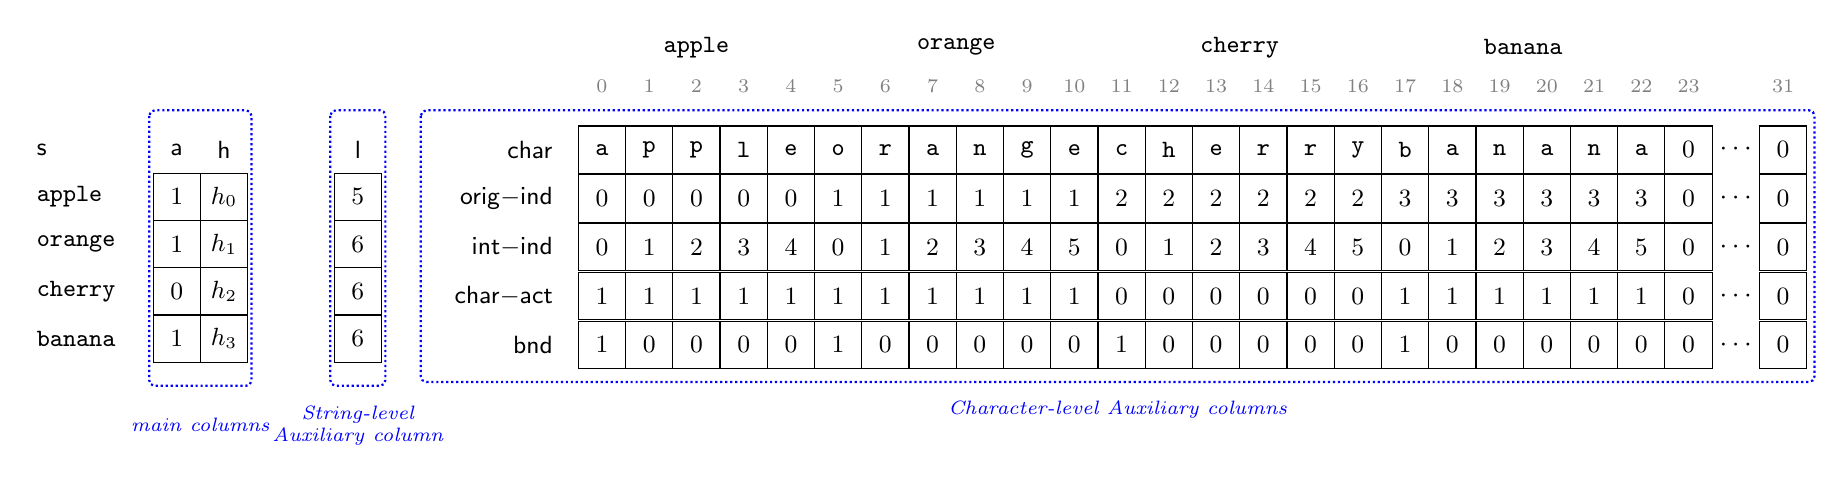
\begin{tikzpicture}[
    cell/.style={draw, minimum size=6mm, inner sep=0pt, font=\small},
    rowlab/.style={font=\small\itshape, anchor=east},
    hd/.style={font=\small\bfseries}
  ]

  %==================== Panel 1: string-level columns ====================
  \node[hd, anchor=west] at (-0.6,5.2) {$\mathsf{s}$};
  \node[hd] at (1.3,5.2) {$\mathsf{a}$};
  \node[hd] at (1.9,5.2) {$\mathsf{h}$};
  \node[hd] at (3.6,5.2) {$\mathsf{l}$};

  % i / string / length / a_h ; row 2 ("cherry") is inactive.
  \foreach \i/\s/\ll/\ah in {0/apple/5/1, 1/orange/6/1, 2/cherry/6/0, 3/banana/6/1}{
    \pgfmathsetmacro{\yy}{4.6 - \i*0.6}
    \node[font=\small\ttfamily, anchor=west] at (-0.6,\yy) {\s};
    \node[cell] at (1.3,\yy) {\ah};
    \node[cell] at (1.9,\yy) {$h_{\i}$};
    \node[cell] at (3.6,\yy) {\ll};
  }

  % dotted box bundling the main column (its activator and hash data)
  \draw[blue, thick, densely dotted, rounded corners=2pt] (0.95,5.7) rectangle (2.25,2.2);
  \node[font=\scriptsize\itshape, blue] at (1.6,1.7) {main columns};

  % dotted box around the string-level auxiliary column (length)
  \draw[blue, thick, densely dotted, rounded corners=2pt] (3.25,5.7) rectangle (3.95,2.2);
  \node[font=\scriptsize\itshape, blue, align=center] at (3.6,1.7) {String-level\\Auxiliary column};

  %==================== Panel 2: character-level columns (placed to the right) ====================
  \begin{scope}[xshift=6.7cm, yshift=5.2cm]
  % group (string) labels above the char row
  \foreach \cx/\nm in {2/apple, 7.5/orange, 13.5/cherry, 19.5/banana}{
    \node[font=\small\ttfamily] at (\cx*0.6, 1.30) {\nm};
  }

  % row labels
  \node[rowlab] at (-0.5, 0.00){$\mathsf{char}$};
  \node[rowlab] at (-0.5,-0.62){$\mathsf{orig\text{-}ind}$};
  \node[rowlab] at (-0.5,-1.24){$\mathsf{int\text{-}ind}$};
  \node[rowlab] at (-0.5,-1.86){$\mathsf{char\text{-}act}$};
  \node[rowlab] at (-0.5,-2.48){$\mathsf{bnd}$};

  % pos / char / orig / o / a_c / s_b ; cherry (orig 2) is inactive so a_c=0 there.
  \foreach \x/\ch/\og/\oo/\ac/\sb in {
     0/a/0/0/1/1,  1/p/0/1/1/0,  2/p/0/2/1/0,  3/l/0/3/1/0,  4/e/0/4/1/0,
     5/o/1/0/1/1,  6/r/1/1/1/0,  7/a/1/2/1/0,  8/n/1/3/1/0,  9/g/1/4/1/0, 10/e/1/5/1/0,
    11/c/2/0/0/1, 12/h/2/1/0/0, 13/e/2/2/0/0, 14/r/2/3/0/0, 15/r/2/4/0/0, 16/y/2/5/0/0,
    17/b/3/0/1/1, 18/a/3/1/1/0, 19/n/3/2/1/0, 20/a/3/3/1/0, 21/n/3/4/1/0, 22/a/3/5/1/0}{
    \pgfmathsetmacro{\px}{\x*0.6}
    \node[font=\scriptsize, gray] at (\px,0.80) {\x};
    \node[cell] at (\px, 0.00) {\texttt{\ch}};
    \node[cell] at (\px,-0.62) {\og};
    \node[cell] at (\px,-1.24) {\oo};
    \node[cell] at (\px,-1.86) {\ac};
    \node[cell] at (\px,-2.48) {\sb};
  }

  % padding tail: one padding slot, an ellipsis, then the final index
  % (31 = last cell of the size-32 hypercube that M=23 pads up to).
  \node[font=\scriptsize, gray] at (23*0.6,0.80) {23};
  \foreach \yy in {0.00,-0.62,-1.24,-1.86,-2.48}{
    \node[cell] at (23*0.6,\yy) {0};
  }
  \foreach \yy in {0.00,-0.62,-1.24,-1.86,-2.48}{
    \node at (24*0.6,\yy) {$\cdots$};
  }
  \node[font=\scriptsize, gray] at (25*0.6,0.80) {31};
  \foreach \yy in {0.00,-0.62,-1.24,-1.86,-2.48}{
    \node[cell] at (25*0.6,\yy) {0};
  }

  % dotted box around the character-level auxiliary columns
  \draw[blue, thick, densely dotted, rounded corners=2pt] (-2.3,0.50) rectangle (15.4,-2.95);
  \node[font=\scriptsize\itshape, blue] at (6.55,-3.3) {Character-level Auxiliary columns};
  \end{scope}

\end{tikzpicture}%
}
\caption{String arithmetization of a four-row column
$\col=(\texttt{apple},\texttt{orange},\texttt{cherry},\texttt{banana})$ with
\texttt{cherry} inactive.}
\label{fig:string-arith-example}
\ifsp\end{figure*}\else\end{figure}\fi




    \parhead{Dropping Auxiliary Columns}
    The final result check needs only the hash column for the opening process, so the auxiliary columns need not be carried all the way through the plan. Deciding \emph{how long} to keep them matters for efficiency: every extra column makes the downstream operations more expensive, especially the character-level columns, which can be far larger than the original string column. The best place to drop them is the earliest point past which the plan performs no further white-box string operation.

    This motivates the planner to push string-filtering operations as far down the plan as possible, so the auxiliary columns can be released early. As \cref{fig:like-query-plans} illustrates, such push-down is possible in some plans but not in others. Plan~(a) applies a \textsc{not like} predicate to \texttt{o\_comment} above a \textsc{left join}: since the join's right input is nullable, filtering the base \texttt{orders} table is not equivalent to filtering after the join, so the predicate is stuck above the join and the string auxiliary columns must be carried through it. Plans~(b) and~(c), by contrast, apply a \textsc{like} predicate to the base column \texttt{p\_name} across an inner \textsc{join}, where the filter commutes with the join; the optimizer therefore pushes it down to the base scan (b~$\to$~c), letting the auxiliary columns be released before the join.




\ifsp\begin{figure*}[tp]\else\begin{figure}[tp]\fi
\centering
\resizebox{\textwidth}{!}{%
\begin{tikzpicture}[
  op/.style={draw, line width=0.9pt, rounded corners=3pt, align=center, font=\footnotesize, inner sep=5pt, fill=white},
  tbl/.style={draw, dashed, line width=0.8pt, rounded corners=3pt, align=center, font=\footnotesize, inner sep=5pt},
  flow/.style={-{Stealth[length=2.4mm,width=2.2mm]}, line width=1.1pt},
  plab/.style={font=\normalsize}]
  % ===================== Plan (a): LEFT JOIN + NOT LIKE filter =====================
  \node[tbl] (a_cust) at (-1.2,0) {\ttfamily customer};
  \node[tbl] (a_ord)  at (1.2,0)  {\ttfamily orders};
  \node[op]  (a_join) at (0,2.2)  {\textbf{Left Join}\\[1pt]\ttfamily c\_custkey = o\_custkey};
  \node[op]  (a_flt)  at (0,4.3)  {\textbf{Filter}\\[1pt]\ttfamily o\_comment NOT LIKE\\ \ttfamily '\%special\%requests\%'};
  \node[tbl] (a_res)  at (0,6.1)  {res};
  \draw[flow] (a_cust) -- (a_join);
  \draw[flow] (a_ord) -- (a_join);
  \draw[flow] (a_join) -- (a_flt);
  \draw[flow] (a_flt) -- (a_res);
  \node[plab] at (0,-1.2) {(a) Left join with \textsc{not like} filter};
  % ---- group (a): single left-join-query plan ----
  \draw[gray!65, dash pattern=on 4pt off 2pt, line width=1pt, rounded corners=10pt]
       (-3.3,-1.9) rectangle (3.3,9.5);
  % ===================== Plans (b),(c): grouped, shifted left to sit closer to (a) =====================
  \begin{scope}[xshift=-1.7cm]
  \node[tbl] (b_line) at (7.0,0)   {\ttfamily lineitem};
  \node[tbl] (b_part) at (9.4,0)   {\ttfamily part};
  \node[op]  (b_join) at (8.2,2.2) {\textbf{Join}\\[1pt]\ttfamily l\_partkey = p\_partkey};
  \node[op]  (b_flt)  at (8.2,4.3) {\textbf{Filter}\\[1pt]\ttfamily p\_name LIKE '\%green\%'};
  \node[op]  (b_proj) at (8.2,6.2) {\textbf{Project}\\[1pt]\ttfamily l\_orderkey, p\_name};
  \node[tbl] (b_res)  at (8.2,8.0) {res};
  \draw[flow] (b_line) -- (b_join);
  \draw[flow] (b_part) -- (b_join);
  \draw[flow] (b_join) -- (b_flt);
  \draw[flow] (b_flt) -- (b_proj);
  \draw[flow] (b_proj) -- (b_res);
  \node[plab] at (8.2,-1.2) {(b) Naive plan};
  % ===================== Plan (c): filter pushdown =====================
  \node[tbl] (c_line) at (13.9,0)  {\ttfamily lineitem};
  \node[tbl] (c_part) at (17.4,0)  {\ttfamily part};
  \node[op]  (c_flt)  at (17.4,2.2){\textbf{Filter}\\[1pt]\ttfamily p\_name LIKE '\%green\%'};
  \node[op]  (c_join) at (15.65,4.3){\textbf{Join}\\[1pt]\ttfamily l\_partkey = p\_partkey};
  \node[op]  (c_proj) at (15.65,6.2){\textbf{Project}\\[1pt]\ttfamily l\_orderkey, p\_name};
  \node[tbl] (c_res)  at (15.65,8.0){res};
  \draw[flow] (c_part) -- (c_flt);
  \draw[flow] (c_flt) -- (c_join);
  \draw[flow] (c_line) -- (c_join);
  \draw[flow] (c_join) -- (c_proj);
  \draw[flow] (c_proj) -- (c_res);
  \node[plab] at (15.65,-1.2) {(c) Filter-pushdown plan};
  % ===================== group (b)+(c): equivalent plans for one query =====================
  \draw[gray!65, dash pattern=on 4pt off 2pt, line width=1pt, rounded corners=10pt]
       (5.5,-1.9) rectangle (20.1,9.5);
  \draw[-{Stealth[length=3mm,width=3mm]}, line width=1.4pt, gray!55]
       (10.7,4.3) -- node[above=1pt, font=\footnotesize, text=black, align=center]
       {optimize\\ \scriptsize(filter push-down)} (13.4,4.3);
  \end{scope}
\end{tikzpicture}}
\caption{Two \textsc{like} query plans: the filter in~(a) cannot be pushed below the join, whereas the one in~(b,c) can (b~$\to$~c).}
\label{fig:like-query-plans}
\ifsp\end{figure*}\else\end{figure}\fi
